\chapter{Development of the chosen solutions [DONE]}

Once we have defined what we want to do in the previous chapter, \textbf{Methodology, Considerations, and Decisions on Alternative Solutions}, it is time to get to work.

\section{Graphic interface}

One important point is to provide a GUI (\textit{Graphical User Interface}) that is intuitive and easy to use. Since Python is being used for development, the chosen solution is to use the Tkinter\cite{Tkinter} library for the window and page system, and the Matplotlib\cite{Matplotlib} library to display graphical results of certain analysis algorithms.

As Tkinter works, all actions that need to be triggered or modified through user interaction must be handled inside a function. Therefore, the way this library operates is by calling predefined functions in response to any user interaction.

First, we need to define the graphical architecture, where each module will be integrated into the graphical user interface. Since the program functions as a set of tools, we must define where each tool will be placed within the interface.

These tools can be divided into two important groups, which will also correspond to two separate windows accessible from the root window:

\begin{itemize}
	\item \textbf{Analysis Window:} This window will contain the tools that need to receive sound from both the external input and the system input (Input from System). It will then display the results of the analysis performed on those signals.
	\item \textbf{DSP Window:} This window, also called the \textbf{"Correction Window"}, contains the tools that receive sound from the external input, as well as data indicating how the signal should be processed, and then send the processed signal to the output (Output to System).
\end{itemize}

Each of these two windows will be divided into pages, with each page containing a specific tool. Additionally, a settings window is needed, where the user can set global parameters. With all of this, we arrive at the following GUI scheme:

\begin{figure}[H]
	\begin{center}
		\vspace{-2mm}
		\tikzsetnextfilename{GUI_path}
		\begin{tikzpicture}[node distance=30mm,on grid,auto, scale=1, bend angle=45]
			
			every node/.style={font=\small};
			
			\node (q_root) [draw, rectangle, minimum size=1cm] {ROOT WINDOW};
			%\node (null_ext) [right=of q_ext] {};
			\node (q_ana) [draw, rectangle, minimum size=1cm, xshift=-3cm, below left=of q_root]{ANALYSIS WINDOW};
			\node (q_dsp) [draw, rectangle, minimum size=1cm, xshift=3cm, below right=of q_root]{DSP WINDOW};
			\node (q_set) [draw, rectangle, minimum size=1cm, yshift=1cm, below=of q_root]{SETTINGS WINDOW};
			\node (q_dev) [draw, rectangle, minimum size=1cm, xshift=2cm, yshift=1cm, below=of q_set]{Device Settings Page};
			\node (q_aud) [draw, rectangle, minimum size=1cm, xshift=-2cm, yshift=1cm, below=of q_set]{Audio Settings Page};
			\node (q_eq) [draw, rectangle, minimum size=1cm, yshift=-1cm, below=of q_dsp]{EQ Page};
			\node (q_ft) [draw, rectangle, minimum size=1cm, yshift=-3cm, below left=of q_ana]{FT Page};
			\node (q_31) [draw, rectangle, minimum size=1cm, right=of q_ft]{31 Bands Page};
			\node (q_del) [draw, rectangle, minimum size=1cm, right=of q_31]{Delay Page};
			
			\draw[blue, very thick, ->] (q_root) edge node {} (q_ana);
			\draw[blue, very thick, ->] (q_root) edge node {} (q_set);
			\draw[blue, very thick, ->] (q_root) edge node {} (q_dsp);
			\draw[green, very thick, ->] (q_dsp) edge node {} (q_eq);
			\draw[green, very thick, ->] (q_set) edge node {} (q_aud);
			\draw[green, very thick, ->] (q_set) edge node {} (q_dev);
			\draw[green, very thick, ->] (q_ana) edge [bend right=10] node {} (q_ft);
			\draw[green, very thick, ->] (q_ana) edge [bend right=12.5] node {} (q_31);
			\draw[green, very thick, ->] (q_ana) edge [bend right=15] node {} (q_del);

			
		\end{tikzpicture}
		\vspace{-2mm}
	\end{center}
	\caption{GUI window schematic}
\end{figure}

To make coding a bit easier, I will take advantage of the different pages to split the code across multiple Python files. In total, there are five files:

\begin{itemize}
	\item \textbf{rta+c.py:} This is the root file that contains all initial instructions and the root window. It is the file that must be executed to start the program. Its name stands for \textbf{Real Time Analysis plus Correction}, which is also the name of the program.
	\item \textbf{settings.py:} This file contains the settings window and its associated pages.
	\item \textbf{dsp.py:} This file contains the DSP (correction) window.
	\item \textbf{analysis.py:} This file contains the analysis window and all its pages.
	\item \textbf{config.py:} This file declares some important variables that must be accessible from anywhere in the program. It does not contain any GUI-related elements.
\end{itemize}

Since the GUI layer is responsible for executing most of the program’s modules, each window’s file also contains all the necessary functions for analysis, processing, and plotting. In addition, all pages follow, as much as possible, the same structure in order to maintain the program’s logic and readability. This structure is based on three parts:

\begin{enumerate}
	\item \textbf{Initialize:} This section initializes the objects needed, sets up the plots with empty data, and defines the labels that will be displayed on the page.
	\item \textbf{Update:} A function that contains the analysis algorithms, draws data on the plots, or runs DSP algorithms. This update function is called in every iteration of the algorithm loop using Tkinter methods.
	\item \textbf{Control:} This final part contains the control parameters, flags, and buttons that affect the update function.
\end{enumerate}

One very important aspect of using Tkinter is object management. By default, common Python classes may not work properly under certain GUI rendering conditions. To avoid this, when an object needs to be accessible from any page of the GUI, I use three different solutions: use of \textit{config.py} as a shared configuration module containing predefined objects, which can be accessed from anywhere by importing this file; use of \textit{global} and \textit{nonlocal} objects inside the same window; and use of Tkinter classes such as \texttt{tkinter.IntVar}.

Finally, even though Tkinter offers a default way to close windows using the "X" symbol in the top left corner of the window, it does not always work properly—it may simply erase the window but not stop the process that is running from that window. To correctly close any window, it is important to define a close function. This function will be executed when the user clicks the "X" symbol, replacing the default function.

\begin{minted}[label=\texttt{ipython}]{python3}
	"""
	In this case, this is the function that closes the root window and, as a consequence, the entire program.
	"""
	
	# Close all
	def on_close_all():
		config.update_enabled = False # Prevent all periodic updates
		stop_global_stream()  # Ensure the stream is stopped
	
		time.sleep(0.5)
		root.destroy()
	
	root.protocol("WM_DELETE_WINDOW", on_close_all)
	
\end{minted}



\section{Signal Path}

To perform any kind of analysis or signal processing, the first thing we need is data—more specifically, signal data captured from the sound card. This data is sent to different modules so that each one can carry out its specific task. Additionally, in the case of the correction module, it is necessary to send output data back to the sound card (the corrected signal). Additionally, there will be non-signal data containing the results of the analysis, which will be sent to the DSP (\textit{Digital Signal Processor}) or the correction window.

\begin{figure}[H]
	\begin{center}
		\vspace{-2mm}
		\tikzsetnextfilename{general_path}
		\begin{tikzpicture}[node distance=30mm,on grid,auto, scale=1, bend angle=45]
			
			every node/.style={font=\small};
			
			\node (q_ext) {External Input};
			\node (null_ext) [right=of q_ext] {};
			\node (q_ana) [draw, rectangle, minimum size=1cm, below right=of null_ext]{Analysis Window};
			\node (q_dsp) [draw, rectangle, minimum size=1cm, above right=of null_ext]{DSP Window};
			\node (q_out) [right=of q_dsp, xshift=2cm]{Output to System};
			\node (q_inp) [right=of q_ana, xshift=2cm]{Input form System};
			
			
			%\node (q_delay) [draw, rectangle, minimum size=1cm, right=of null_init] {Delay Buffer};
			%\node (q_ext) [draw, rectangle, minimum size=1cm, above right=of q_delay, xshift=2cm] {Filtering and RMS Calculation of External Input};
			%\node (q_in_sys) [draw, rectangle, minimum size=1cm, below right=of q_delay, xshift=2cm] {Filtering and RMS Calculation of Input from System};
			%\node (q_diff) [draw, rectangle, minimum size=1cm, right=of q_delay, xshift=4cm] {Difference calculation};	
			
			\draw[blue, very thick, ->] (q_ext) edge node {} (q_ana);
			\draw[blue, very thick, ->] (q_ext) edge node {} (q_dsp);
			\draw[blue, very thick, ->] (q_dsp) edge node {} (q_out);
			\draw[blue, very thick, ->] (q_inp) edge node {} (q_ana);
			\draw[green, dotted, very thick, ->] (q_ana) edge [bend right=10] node {Data} (q_dsp);
			%\draw[blue, dotted, very thick, ->] (q_delay) edge[bend right=10] node {1 channel} (q_ext);
			%\draw[blue, dotted, very thick, ->] (q_delay) edge[bend right=10] node {1 channel} (q_in_sys);
			%\draw[green, very thick, ->] (q_ext) edge[bend right=10] node {Analysis Data} (q_diff);
			%\draw[green, very thick, ->] (q_in_sys) edge[bend right=10] node {Analysis Data} (q_diff);
			
		\end{tikzpicture}
		\vspace{-2mm}
	\end{center}
	\caption{Basic representation of the required signal path}
\end{figure}

To achieve real-time processing, we must manage a constant flow of data. For this purpose, I will use a stream-style data management approach, which consists of capturing small blocks of data, processing them, and continuously sending the results. To capture and send this stream to and from the sound card, the Sounddevice library \cite{sounddevice} will be used.

To simplify things, the two required inputs—\textbf{External Input} and \textbf{Input from System}—will be handled using a single input stream, while the output—\textbf{Output to System}—will be managed through a separate, independent output stream. All streams will share the same parameters, such as bit depth, sample rate, and block size. However, the audio device and channel parameters will be independently set for each stream. In the case of the input stream, each input channel must also be configured separately.

Once the streams are running and managed from the root window, we need to handle the data coming from the input streams and the data to be sent to the output stream. To achieve this, I will use one input buffer for both input channels and a separate output buffer. These buffers must be accessible to all tool modules in the program and will be locked whenever a module accesses them, in order to prevent simultaneous reads and writes.

\begin{figure}[H]
	\begin{center}
		\vspace{-2mm}
		\tikzsetnextfilename{stream_path}
		\begin{tikzpicture}[node distance=30mm,on grid,auto, scale=1, bend angle=45]
			
			every node/.style={font=\small};
			
			\node (q_ext) {External Input};
			%\node (null_ext) [right=of q_ext] {};
			\node (q_in_st) [draw, rectangle, minimum size=1cm, right=of q_ext, yshift=-1cm, xshift=1cm]{Input Stream};
			\node (q_inp) [left=of q_in_st, yshift=-1cm, xshift=-1cm]{Input form System};
			\node (q_inp_bf) [draw, rectangle, minimum size=1cm, right=of q_in_st]{Input Buffer};
			\node (q_mod) [draw, rectangle, minimum size=1cm, below right=of q_inp_bf]{Tools Modules};
			\node (q_out_bf) [draw, rectangle, minimum size=1cm, below left=of q_mod]{Output Buffer};
			\node (q_out_st) [draw, rectangle, minimum size=1cm, left=of q_out_bf]{Output Stream};
			\node (q_out) [left=of q_out_st, xshift=-1cm]{Output to System};
						
			\draw[blue, very thick, ->] (q_ext) edge node {} (q_in_st);
			\draw[blue, very thick, ->] (q_inp) edge node {} (q_in_st);
			\draw[blue, very thick, ->] (q_in_st) edge node {} (q_inp_bf);
			\draw[green, very thick, ->] (q_inp_bf) edge [bend left=30] node {} (q_mod);
			\draw[green, very thick, ->] (q_inp_bf) edge [bend left=50] node {to multiple modules} (q_mod);
			\draw[green, very thick, ->] (q_mod) edge [bend left=40] node {from one module} (q_out_bf);
			\draw[blue, very thick, ->] (q_out_bf) edge node {} (q_out_st);
			\draw[blue, very thick, ->] (q_out_st) edge node {} (q_out);
			
			
		\end{tikzpicture}
		\vspace{-2mm}
	\end{center}
	\caption{Stream management}
\end{figure}

\section{Settings page}

In order to be flexible with hardware, we need a settings window where we can tell the program which sound card, which channel, and which parameters we want to use. These parameters will also affect the resolution and fidelity of the analysis and processing, according to the sound card’s capabilities.

I will splitt setting window in tow pages:
 \begin{itemize}
 	\item \textbf{Device Settings:} Where we can define which sound card and which channels we want to use.
 	\item \textbf{Audio Settings:} Where we can define which audio parameters we want to use.
 \end{itemize}

\subsection{Device Settings}

I will use sounddevice methods to identify which sound cards and channels are available, and filter them into inputs and outputs. Then, using a questionnaire-style interface, I will let the user select which sound card and which channel they want for each required signal using a dropdown menu.

At the bottom of the page, there will be a "Confirm" button that performs some basic checks, such as verifying that the "external input" and the "input from system" are not the same input channel. Then, it will display a green message if the settings are applied successfully, or a red one if something goes wrong. Finally, it will update the values and labels on the root window to indicate which channels are currently selected.

\begin{figure}[H]
	\centering
	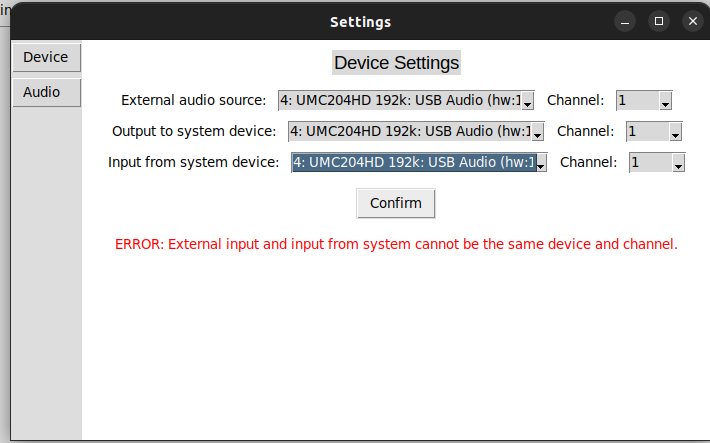
\includegraphics[width=0.8
	\linewidth]{Figures/DevSet.png}
	\caption{Device Settings page showing a red message because the user selected an invalid configuration.}
	\label{fig:Device Settings}
\end{figure}

\subsection{Audio Settings}

On this page, just like in the previous one, I will use a questionnaire-style interface with dropdown menus to define the Sample Rate, Bit Depth, and Block Size to be used.

For the Sample Rate and Bit Depth, I will suggest the most common values — such as 44,100 Hz, 48,000 Hz, 96,000 Hz, and 192,000 Hz for the sample rate, and 16, 24, and 32 bits for bit depth. However, the user is free to enter any value. The same applies to the Block Size.

At the bottom of the page, there is also a "Confirm" button, similar to the one in the "Device Settings" page. It performs basic checks, updates the selected values, and displays a message: green if everything is OK, orange in case of a warning (it applies the changes but alerts the user when a non-recommended or uncommon value is entered), and red if the Block Size is not a power of two — something required for the algorithms to work properly.

\begin{figure}[H]
	\centering
	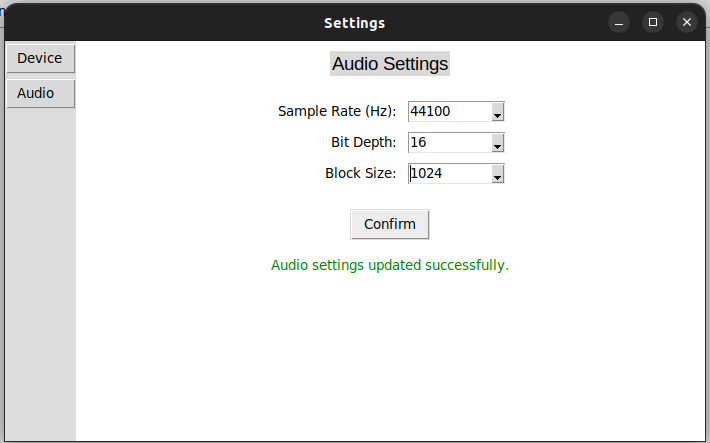
\includegraphics[width=0.8
	\linewidth]{Figures/AudSet.png}
	\caption{Audio Settings page showing a green message.}
	\label{fig:Audio Settings}
\end{figure}



\section{Acoustics analysis}

This part represents the most complex part of the project, so it consists of different sets of tools, and some of them have to interact with each other. As was said before, each tool is inside an independent page.

So, first, apart from initial definitions, drawings, and labels, we need solid page management to ensure correct operation (without processes interfering with each other). The idea to develop is to close and erase everything related to one page every time the user changes pages, and then the new page will be executed. If something needs to be saved for later use on another page, it will be stored in a globally accessible object, managed from within each page. For example, the number of samples used to delay the external input signal is saved in the \textit{config.py} module.

\begin{minted}[label=\texttt{ipython}]{python3}
	"""
	Close and Open Sequence for Page Switching
	"""
	
	# Destroy and unload current pages
	config.update_enabled = False
	time.sleep(0.3) #Give time for end whatever was executing
	
	# Close all matplotlib figures to prevent memory leak
	for fig in plt.get_fignums():
		plt.close(fig)
	print("[INFO] Killed previous plots")
	
	for name, frame in pages.items():
		frame.pack_forget()
		frame.destroy()  # Destroy the frame's widgets
	pages.clear()
	loaded_pages.clear()
	print("[INFO] Cleared previous pages")
	
	# Destroy any active page
	for name in list(pages.keys()):
		pages[name].destroy()  # remove from memory
		del pages[name]
		del loaded_pages[name]
	print("[INFO] Deleted previous pages")
	
	time.sleep(0.3) #Give more time
	
	config.update_enabled = True
	print(page_name)
	
	# Load and show new page
	if page_name == "FT":
		load_ft_page()
	elif page_name == "31 Bands":
		load_31bands_page()
	elif page_name == "Delay":
		load_delay_page()
\end{minted}

All signal and analysis algorithms are implemented using the \textbf{NumPy}\cite{numpy} and \textbf{SciPy}\cite{scipy_signal} libraries.

\subsection{Spectrogram (FT)}

In studio or live sound situations, a spectrogram shows the energy of different frequencies over time using \textbf{FT} (\textit{Fourier Transform}), displayed in the audible range (between 20 Hz and 20 kHz), and sometimes slightly extended beyond.

In my case, as a starting point, I’m using \texttt{numpy.fft.rfft}, which is the \textbf{RFFT} (\textit{Real Fast Fourier Transform}) function from the NumPy library. It is an efficient variation of the \textbf{FFT} (\textit{Fast Fourier Transform}) designed for real-valued input signals.

In order to achieve good resolution, the processing block size on this page is independent of the one set in the settings pages. It uses at least 100 ms of data (more precisely, the next power-of-two number of samples equivalent to 100 ms). This provides a minimum frequency resolution of 10 Hz.

\begin{figure}[H]
	\centering
	\caption{Frequency Resolution as a Function of Time Window}
	\[
	\Delta f = \frac{1}{T}
	\]
\end{figure}

But before starting the calculations, we first need to prepare the input data through two processes.

First, we have to delay the \textit{External Input} signal to match it with the \textit{Input from System} signal. This is managed using a set of instructions that operate on the delay buffer. Also, if there is not enough data to apply the required delay, the system waits for the next iteration.

\begin{minted}[label=\texttt{ipython}]{python3}
	"""
	Set of Instructions to Manage the Delay Buffer
	"""
	
    # Get delayed data
	if config.delay_samples == 0:
		ext_data = config.delay_buffer[-N_FFT:]
	else:
		ext_data = config.delay_buffer[-(config.delay_samples + N_FFT):-config.delay_samples]

	if ext_data is None or len(ext_data) < N_FFT:
		analysis_window.after(100, update_spectrogram)
		print("[DEBUG] Delayed ext_data too short")
		return
	
\end{minted}

Secondly, I apply a windowing process to the acquired data in order to obtain more pleasant and understandable results to display. It is true that this kind of process slightly alters the final results, but in this case, it can help to better identify peaks that stand out—indicating possible resonances—and valleys, which can indicate cancellations, extra absorption, or a lack of energy in certain frequencies.

After trying several different window functions, I decided to use a \textit{Blackman} window, implemented with the \texttt{numpy.blackman} function from the \textbf{NumPy} library.

After the FT calculations, I apply an averaging algorithm that can be performed either over time or over frequency. Time averaging is particularly useful when using non-varying sounds for frequency analysis to excite the system—for example, constant pink noise—allowing more stable and defined results.

Frequency averaging, on the other hand, is useful when analyzing the high-frequency range. In order to achieve good resolution in the low-frequency range, we often end up with unnecessarily high resolution in the high frequencies, since the data is displayed on a logarithmic scale. Therefore, if the user wants to focus on the high-frequency range, reducing the resolution through frequency averaging can make the visualization clearer and easier to interpret.

The final step is calculate the difference between External Input analysis and Input from System analysis, in order to get frequency response of the system. This is done with a simple resta of Analysis results.

\begin{figure}[H]
	\begin{center}
		\vspace{-2mm}
		\tikzsetnextfilename{FT_page_schem}
		\begin{tikzpicture}[node distance=30mm,on grid,auto, scale=1, bend angle=45]
			
			every node/.style={font=\small};
			
			\node (q_init) [draw, rectangle, minimum size=1cm,] {Input Buffer};
			\node (null_init) [right=of q_init] {};
			\node (q_delay) [draw, rectangle, minimum size=1cm, right=of null_init] {Delay Buffer};
			\node (q_ext) [draw, rectangle, minimum size=1cm, above right=of q_delay, xshift=2cm] {Windowing, FT and Averaging of External Input};
			\node (q_in_sys) [draw, rectangle, minimum size=1cm, below right=of q_delay, xshift=2cm] {Windowing, FT and Averaging of Input from System};
			\node (q_diff) [draw, rectangle, minimum size=1cm, right=of q_delay, xshift=4cm] {Difference calculation};	
			
			\draw[blue, very thick, ->] (q_init) edge node {2 channels} (q_delay);
			\draw[blue, dotted, very thick, ->] (q_delay) edge[bend right=10] node {1 channel} (q_ext);
			\draw[blue, dotted, very thick, ->] (q_delay) edge[bend right=10] node {1 channel} (q_in_sys);
			\draw[green, very thick, ->] (q_ext) edge[bend right=10] node {Analysis Data} (q_diff);
			\draw[green, very thick, ->] (q_in_sys) edge[bend right=10] node {Analysis Data} (q_diff);
			
		\end{tikzpicture}
		\vspace{-2mm}
	\end{center}
	\caption{Diagram of the architecture of the FT page}
\end{figure}

At the end of the page, GUI elements are added for user interaction, allowing the user to set averaging values and to pause or resume the analysis.

\begin{figure}[H]
	\centering
	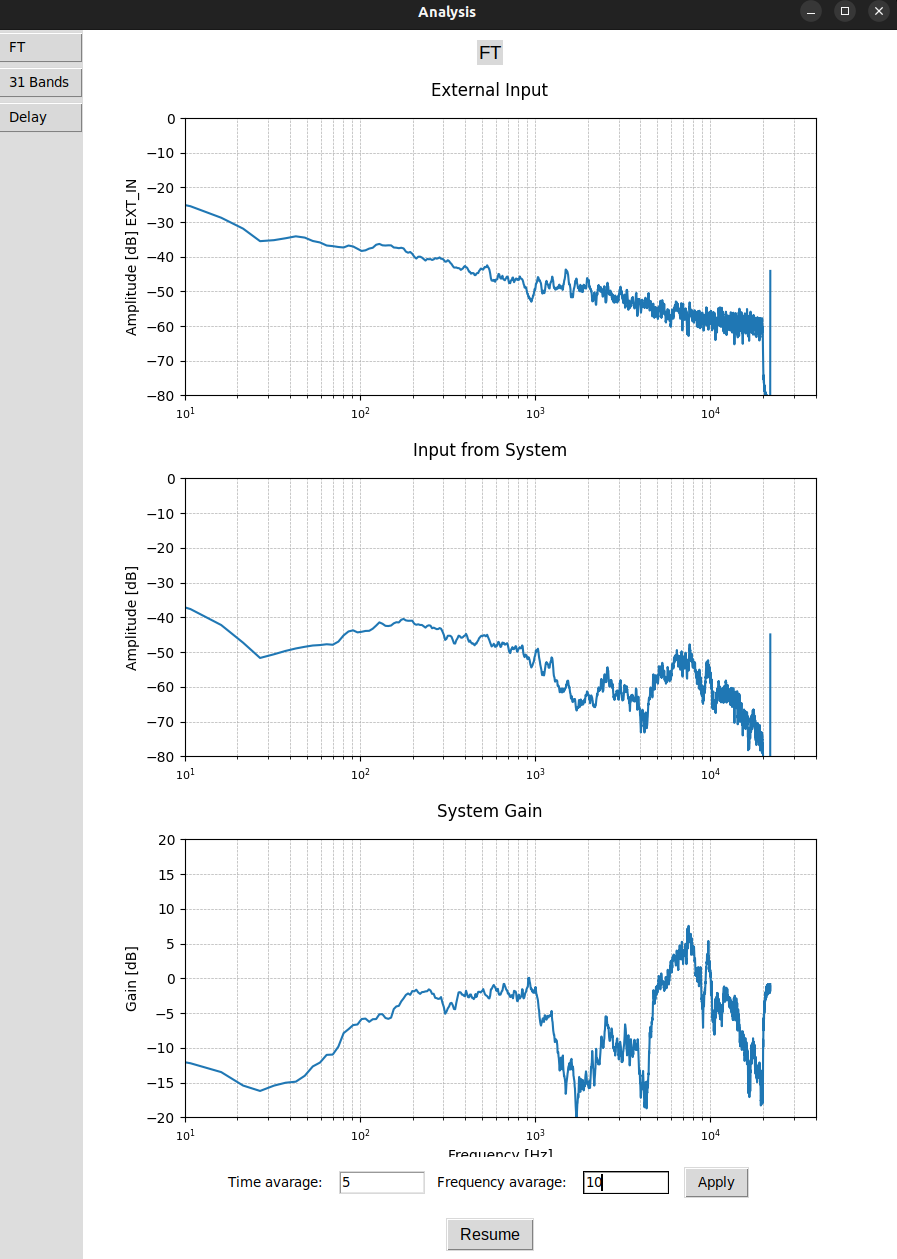
\includegraphics[width=0.7
	\linewidth]{Figures/FT_page.png}
	\caption{Analysis window - FT page.}
	\label{fig:FT Page}
\end{figure}

Figure~\ref{fig:FT Page} shows pink noise in the External Input, the signal captured with a microphone in the Input from System, and their difference, using various averaging options.



\subsection{RTA}

Usually, any form of analysis that is performed in real time can be considered \textbf{RTA} (\textit{Real-Time Analysis}). This includes a wide range of operations such as spectrum monitoring, transfer function measurements, phase and coherence analysis, and more—all happening as the signal flows. However, in my experience, in common usage, when someone refers to "RTA", they are often specifically referring to the classic 31-band graphical spectrum display. Also, the data collected on this page is especially important because it will be used to set the correction parameters. For all of that, this page has been named \textbf{RTA}.



Also, there is another conflict. When someone defines the 31 bands and their bandwidth, it is common to use the definition provided in \textbf{IEC 61260}. However, this standard does not mathematically respect the logarithmic spacing between bands. The 31 bands are defined as 1/3 of an octave per band.

\begin{table}[H]
\centering
\caption{Center frequencies for true 1/3 octave bands and IEC 61260 bands} 

	\scalebox{0.53}{
		\begin{tabular}{|c|c|c|c|c|c|c|c|c|c|c|c|}
			\hline
			1/3 octave & 19.69 & 24.8 & 31.25 & 39.37 & 49.61 & 62.5 & 78.75 & 99.21 & 125 & 157.49 & \\ \hline
			IEC 61260 & 20 & 25 & 31.5 & 40 & 50 & 63 & 80 & 100 & 125 & 160 & \\ \hline
			 & & & & & & & & & & & \\ \hline
			1/3 octave & 198,43 & 250 & 314.98 & 396.85 & 500 & 629.96 & 793.7 & 1000 & 1259.92 & 1587.4 & \\ \hline
			IEC 61260 & 200 & 250 & 315 & 400 & 500 & 630 & 800 & 1000 & 1250 & 1600 & \\ \hline
			 & & & & & & & & & & & \\ \hline
			1/3 octave & 2000 & 2519.84 & 3174.8 & 4000 & 5039.68 & 6349.6 & 8000 & 10079.37 & 12699.21 & 16000 & 20158.74 \\ \hline
			IEC 61260 & 2000 & 2500 & 3150 & 4000 & 5000 & 6300 & 8000 & 10000 & 12500 & 16000 & 20000 \\ \hline
				
		\end{tabular}
	}
\end{table}

\begin{minted}[label=\texttt{ipython}]{python3}
	"""
	In order to obtain the true 1/3 octave values, the following line of code was used with IPython3.
	The results were rounded to the second decimal place.
	"""
	
	[round(1000*2**(band/3), 2) for band in range (-17,14)]
	
\end{minted}

On the other hand, this standard is widely used in many professional devices and software. One important example is the DBX 231s graphic equalizer, which is commonly used in analog processing chains.

\begin{figure}[H]
	\centering
	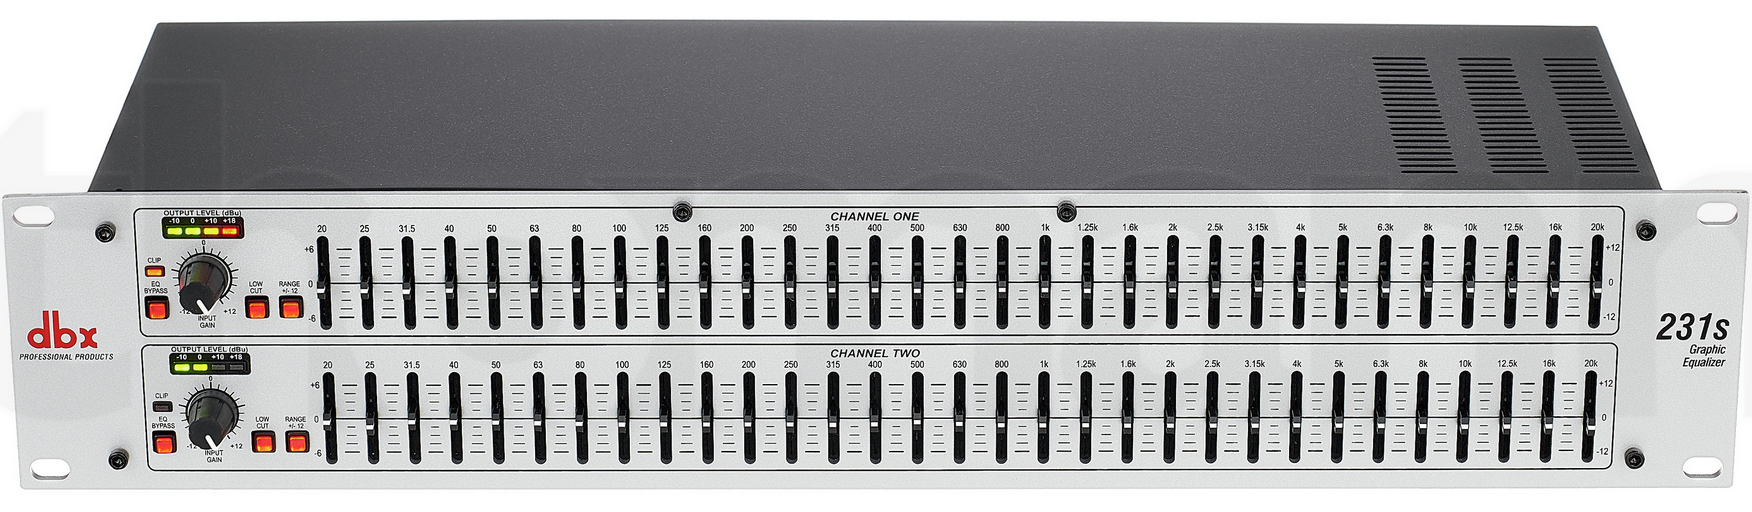
\includegraphics[width=1
	\linewidth]{Figures/DBX_231s.png}
	\caption{Image of the front panel of the DBX 231s \cite{DBX_31s}, where we can observe that the center frequency bands are the same as those defined in IEC 61260.}
	\label{fig:DBX_31s}
\end{figure}

In order to achieve the greatest possible compatibility and coherence with industry standards, I prefer to use the IEC 61260 standard.


The signal path on this page is very similar to the one used on the "FT" page. We have a buffer with two blocks of input data ("Input from external device" and "Input from system").

First, we copy the buffer data to the "delay buffer", where, if needed, the data will be adjusted to make it coincide with the applied delay. If necessary, the adjustment will use data from previous blocks stored in the same "delay buffer".

I created this buffer with the capacity to store 1 second of data, which can be used to apply a maximum delay of (1 - "Block Size in seconds") seconds.

Once the data in the "delay buffer" is adjusted, we can start applying algorithms to perform the analysis.

The algorithm is based on the calculation of RMS (\textit{root mean square}) to obtain the energy for each frequency band, which is divided using filters for each band.


\begin{figure}[H]
	\begin{center}
		\vspace{-2mm}
		\tikzsetnextfilename{RTA_page_schem}
		\begin{tikzpicture}[node distance=30mm,on grid,auto, scale=1, bend angle=45]
			
			every node/.style={font=\small};
			
			\node (q_init) [draw, rectangle, minimum size=1cm,] {Input Buffer};
			\node (null_init) [right=of q_init] {};
			\node (q_delay) [draw, rectangle, minimum size=1cm, right=of null_init] {Delay Buffer};
			\node (q_ext) [draw, rectangle, minimum size=1cm, above right=of q_delay, xshift=2cm] {Filtering, RMS Calculation, and Averaging of External Input};
			\node (q_in_sys) [draw, rectangle, minimum size=1cm, below right=of q_delay, xshift=2cm] {Filtering, RMS Calculation and Averaging of Input from System};
			\node (q_diff) [draw, rectangle, minimum size=1cm, right=of q_delay, xshift=4cm] {Difference calculation};	
			
			\draw[blue, very thick, ->] (q_init) edge node {2 channels} (q_delay);
			\draw[blue, dotted, very thick, ->] (q_delay) edge[bend right=10] node {1 channel} (q_ext);
			\draw[blue, dotted, very thick, ->] (q_delay) edge[bend right=10] node {1 channel} (q_in_sys);
			\draw[green, very thick, ->] (q_ext) edge[bend right=10] node {Analysis Data} (q_diff);
			\draw[green, very thick, ->] (q_in_sys) edge[bend right=10] node {Analysis Data} (q_diff);
			
		\end{tikzpicture}
		\vspace{-2mm}
	\end{center}
	\caption{Diagram of the architecture of the RTA page}
\end{figure}


In this case, I'm not using any kind of windowing. As a starting point, I'm using 4th-order IIR (\textit{infinite impulse response}) Butterworth band-pass filters for each band. All these filters are created using the \texttt{scipy.signal} library \cite{scipy_signal}, which returns SOS (\textit{Second-Order Section}) parameters.

\begin{figure}[H]
	\centering
	\caption{Second-Order Sections for IIR filters with their parameters}
	\[
	H(z) = \frac{b_0 + b_1 z^{-1} + b_2 z^{-2}}{1 + a_1 z^{-1} + a_2 z^{-2}}
	\]
\end{figure}

When the program applies each filter to the signal block, it also calculates the RMS and converts it to a logarithmic scale, which will be plotted on the graph and used to calculate the difference graph.

\begin{figure}[H]
	\centering
	\caption{Root Mean Square to calculate energy from filtered signal}
	\[
	RMS = \sqrt{ \frac{1}{N} \sum_{n=0}^{N-1} x^2[n] }
	\]
\end{figure}

At the end, there is: a pause button, which blocks the update function and can be used to pause the graphics; a save button, to store the current values of the difference graph for later use in the correction window; and a time averaging section that works exactly the same as the averaging section from the FT page, except that it does not include frequency averaging (since it doesn't make sense to apply frequency averaging between bands).

\begin{figure}[H]
	\centering
	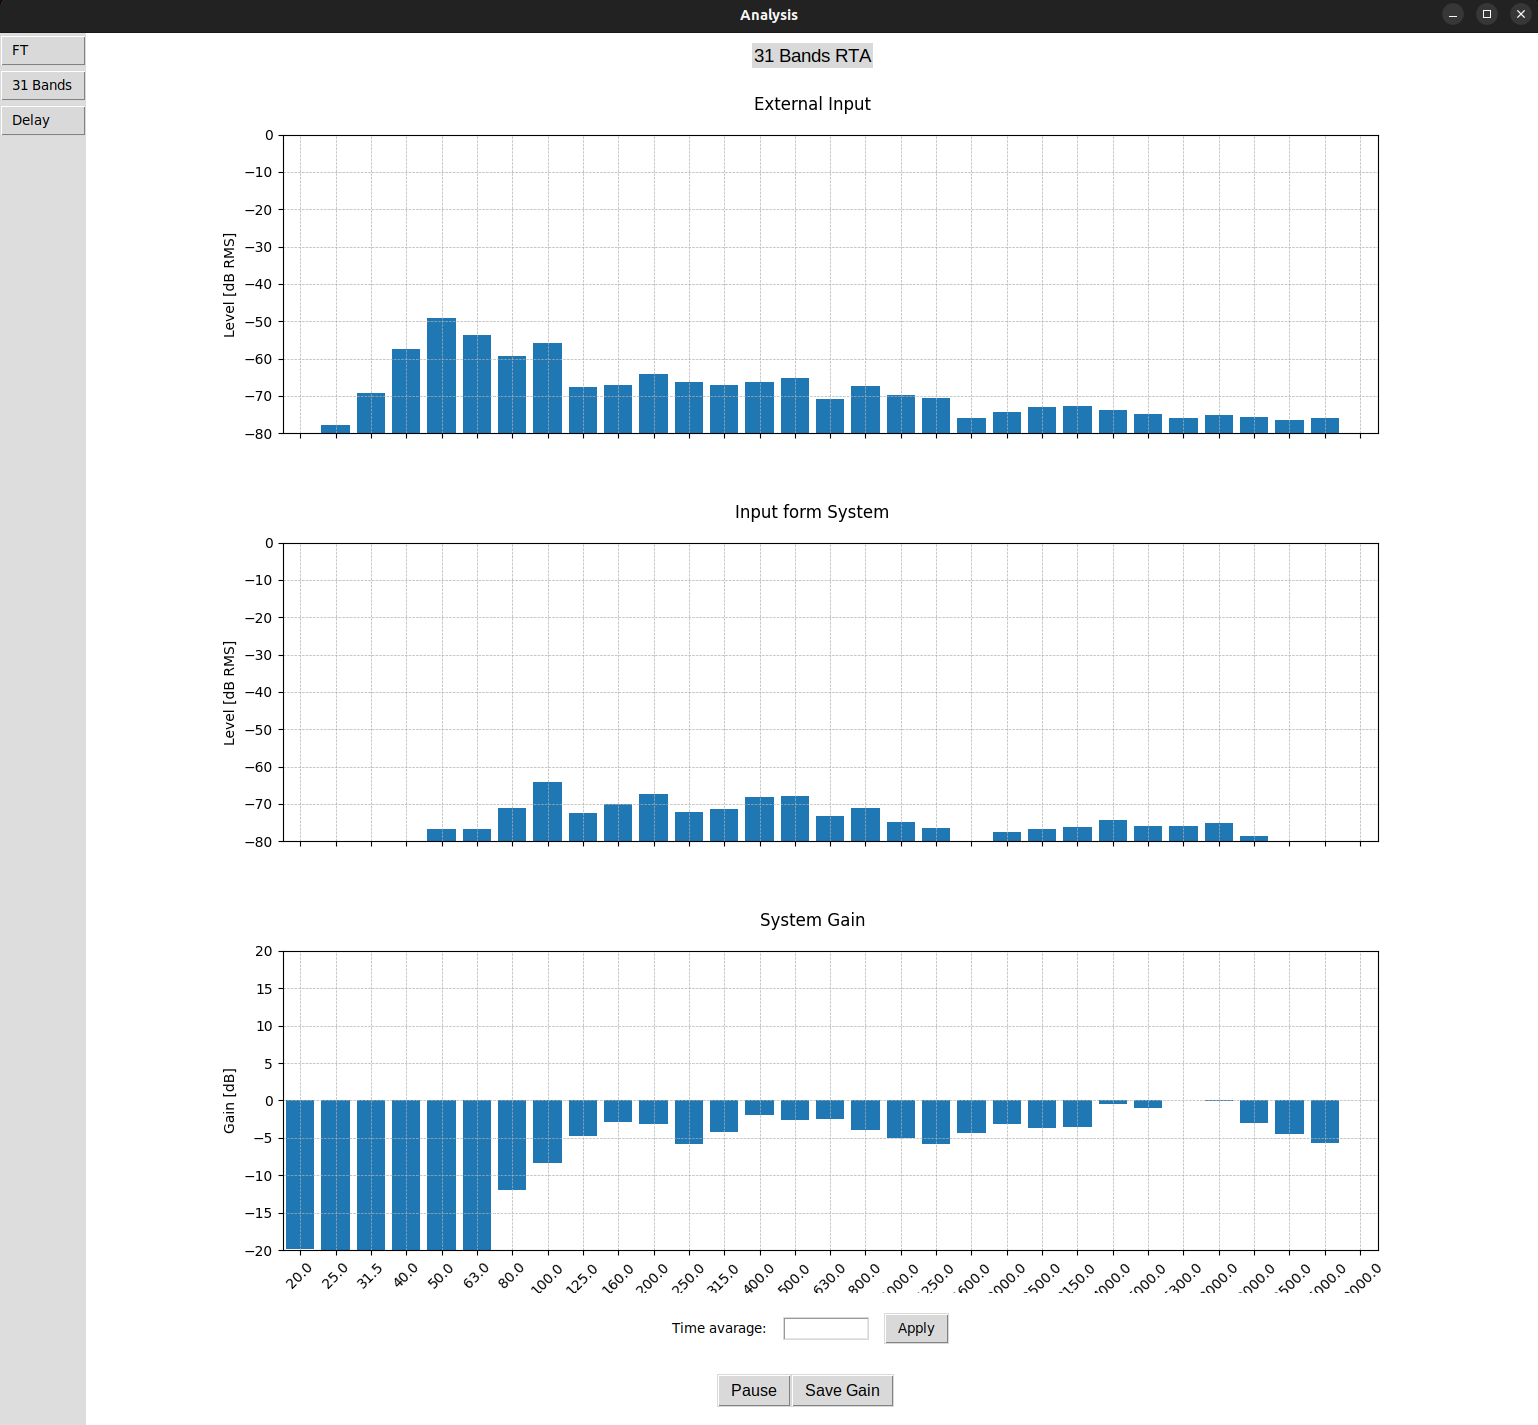
\includegraphics[width=1
	\linewidth]{Figures/RTA_page.png}
	\caption{Analysis window - RTA page.}
	\label{fig:RTA_page}
\end{figure}


\subsection{Delay}

Usually, all systems introduce some delay, primarily caused by the travel time of sound between the speaker and the microphone. However, additional subsystems can also contribute to further delay. In cases where we want to perform analysis in a live situation with music (for example, measuring during a live show), where the excitation signal is not time-invariant in terms of frequency content, it is crucial to synchronize both inputs of the program in order to obtain an accurate representation from the analysis.

As explained in the FT and RTA pages, this synchronization is achieved using a dedicated buffer that allows shifting samples to align the signals. However, this mechanism needs to know how many samples the \textbf{External Input} must be delayed in order to compensate for the delay introduced by the system (\textbf{Input from System}). The main goal of this page is to calculate that delay value.

For this purpose, I will use a correlation algorithm on both input signals to identify where they are most similar. However, to reduce the effect of amplitude changes introduced by the system, I first normalize each signal by its own RMS value before performing the correlation. For the correlation itself, I use the \texttt{scipy.signal.correlate} function from the \textit{SciPy} library.

Once the correlation is obtained, I apply the absolute value to all results to eliminate the effect of possible polatity inversion introduced by the system (since an inverted signal would produce a negative correlation value). Then, I discard results corresponding to delays shorten than -10 ms. In the types of systems this program id designed to analyze, negative delays are physically impossible, as they would imply predicting a future signal. However, I allow a small negative range to help detect potential issues in case something goes wrong.

Now we can search for the maximum value of the correlation, and the position of this maximum will indicate the number of samples to delay. The result will be labeled both in samples and in the equivalent milliseconds. Additionally, I will plot the absolute correlation result to visually assess whether the detection is reliable. If the maximum value stands out clearly from the rest of the correlation, it means a strong and well-defined match has been found. However, if the peak does not stand out much, or if there are multiple peaks of similar value, the result may not be entirely reliable.

\begin{figure}[H]
	\begin{center}
		\vspace{-2mm}
		\tikzsetnextfilename{Delay_page_schem}
		\begin{tikzpicture}[node distance=30mm,on grid,auto, scale=1, bend angle=45]
			
			every node/.style={font=\small};
			
			\node (q_init) [draw, rectangle, minimum size=1cm,] {Input Buffer};
			\node (q_norm) [draw, rectangle, minimum size=1cm, right=of q_init] {Normalize};
			\node (q_cor) [draw, rectangle, minimum size=1cm, right=of q_norm] {Correlation};
			\node (q_abs) [draw, rectangle, minimum size=1cm, right=of q_cor, xshift=2cm] {Absolute, Arange and serach Max};
			
			\draw[blue, very thick, ->] (q_init) edge node {} (q_norm);
			\draw[blue, very thick, ->] (q_norm) edge node {} (q_cor);
			\draw[green, very thick, ->] (q_cor) edge node {} (q_abs);
			
			
		\end{tikzpicture}
		\vspace{-2mm}
	\end{center}
	\caption{Diagram of the architecture of the Delay page}
\end{figure}

At the bottom of the page, I will add a “Pause / Resume” button and an “Apply” button, which saves the delay value in an object accessible to the other analysis pages. Once this parameter is saved, the other pages will automatically start applying the delay to their corresponding analyses.

\begin{figure}[H]
	\centering
	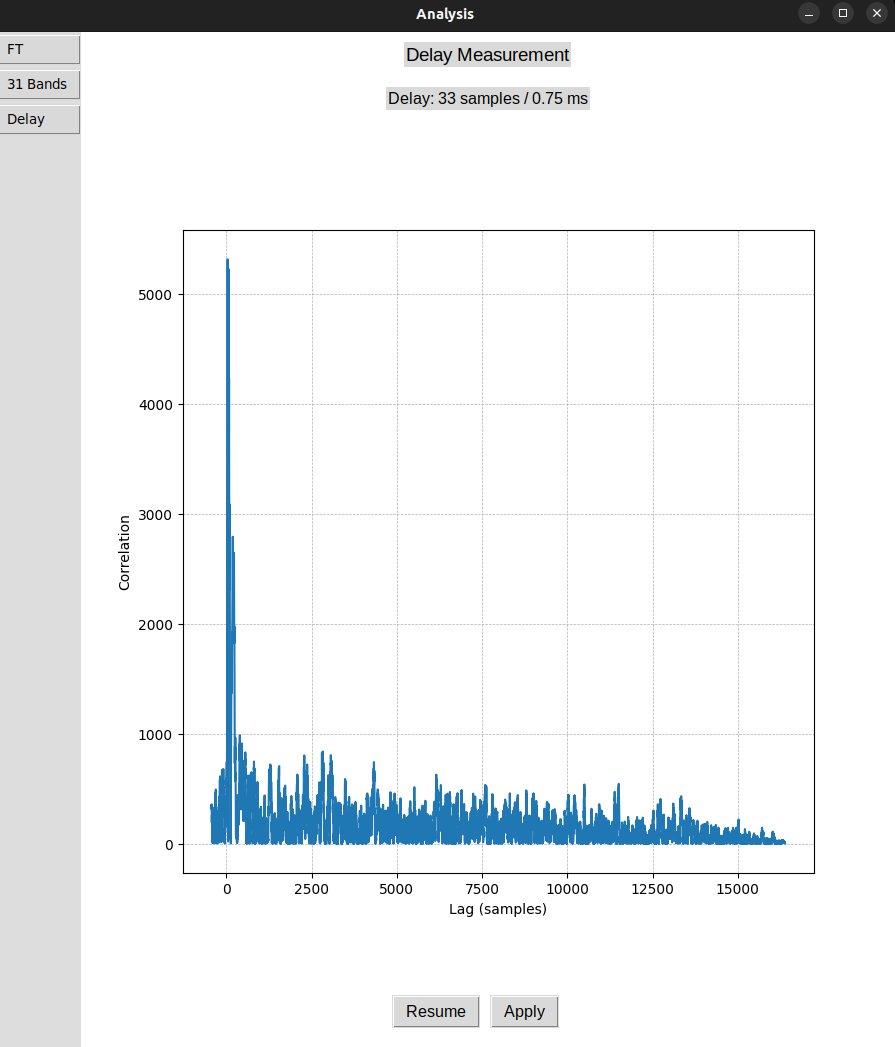
\includegraphics[width=0.7
	\linewidth]{Figures/Delay_page.png}
	\caption{Analysis window - Delay page.}
	\label{fig:Delay_page}
\end{figure}

Figure~\ref{fig:Delay_page} was captured using pink noise, with the microphone placed approximately 25 cm from the speaker, which corresponds to nearly 0.25 ms of delay.


\section{Acoustic correction}

The acoustic correction is based on a \textbf{DSP} (\textit{Digital Signal Processor}) that processes the \textbf{External Input}, aiming to compensate for the imperfections of the analyzed system in order to improve the sound at the listening position. The processed signal is then sent through the \textbf{Output to System}.

This processing is based on a 31-band graphic equalizer using the IEC 61260-defined bands, to ensure consistency with the analysis and with common industry solutions (as explained in the Analysis–RTA section).

Furthermore, it must be able to bypass the processing, in case the user just wants to hear the unprocessed signal. It should also be possible to stop the \textbf{Output to System}, acting as a mute option. To switch between these three states, instead of using separate pages, I implemented a single button that cycles through the “Stop”, “Bypass”, and “EQ” states.

As the output stream is almost always active and continuously reads data from the output buffer, the “Stop” state is implemented by simply writing zeros to the output buffer. In fact, zeros are also the default content of the buffer.

\begin{figure}[H]
	\centering
	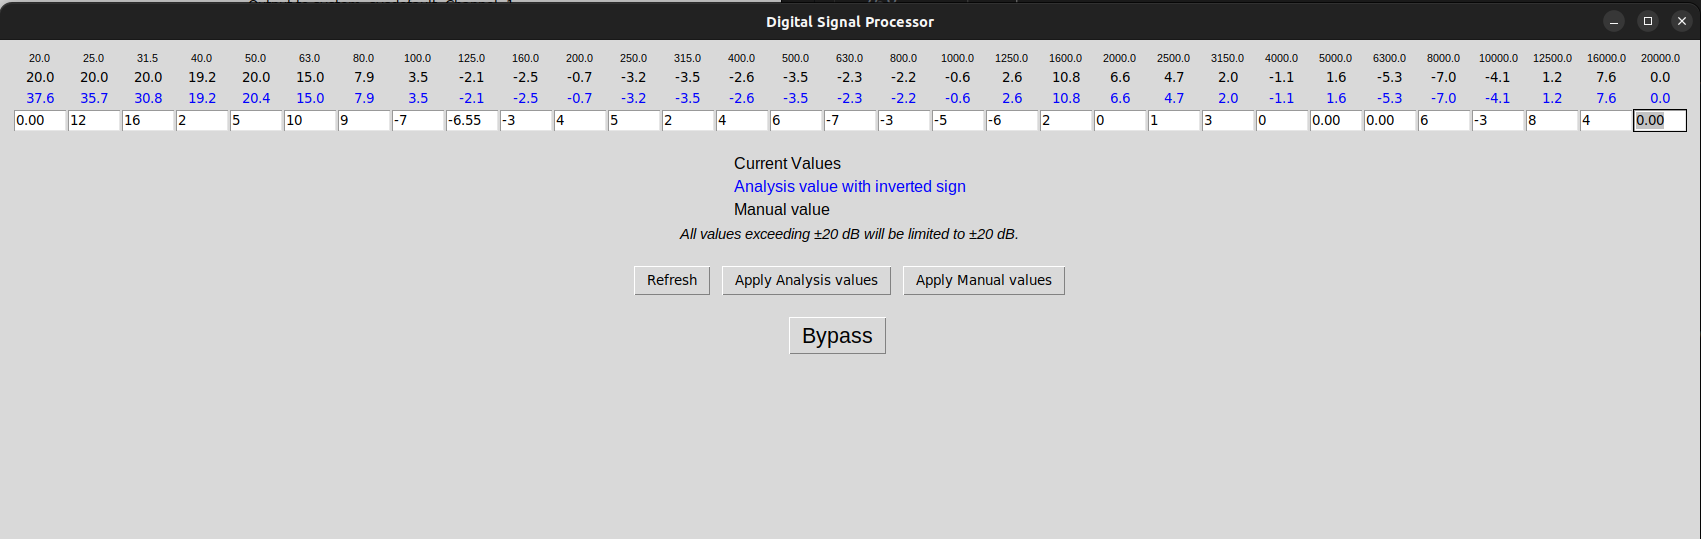
\includegraphics[width=1
	\linewidth]{Figures/DSP_page.png}
	\caption{Correction window - DSP.}
	\label{fig:DSP_page}
\end{figure}

A very important aspect of this page is that it must take the data saved from the Analysis–RTA section and invert it, since compensating the system requires applying the inverse of the measured values. This is done automatically when the page is opened or when the user presses “Refresh.” Additionally, the user has the option to manually enter their own values.


\subsection{Bypass}

When I was developing one of the first versions of the program, I did not use shared buffers—each page managed its own stream, directly reading data from the input stream, processing it as needed, and, if necessary, writing directly to the output stream. For example, this was the code used for the Bypass function at that time: it took data from the input stream, stored it in a temporary buffer used only for this function, and then wrote that buffer to the output stream.

\begin{minted}[label=\texttt{ipython}]{python3}
	"""
	Core part of the code for the Bypass functionality that was working correctly.
	"""
	
	indata, _ = input_stream.read(block_size.get())
	buffer[:] = indata[:, ext_in_ch.get() - 1]
	out_block = np.zeros((block_size.get(), output_stream.channels), dtype='float32')
	out_block[:, out_to_sys_ch.get() - 1] = buffer
	output_stream.write(out_block)
\end{minted}

This meant that every tool or page had to have its own input and output stream. However, while implementing the Bypass feature, I quickly realized that I couldn't use different streams simultaneously for the same physical input or output channels (for example, Bypass and FT analysis at the same time), because the Sounddevice library does not allow this.

Then, I switched to the current signal and path management approach, as explained earlier in the \textbf{Signal Path} section. I'm explaining this because this is the point where the Bypass functionality stopped working properly. The important issue that appeared will be discussed later in the \textbf{Results} chapter.

Nevertheless, the new signal path allows the program to simultaneously have a working Bypass while updating the FT analysis.

Specifically, the idea behind the Bypass is to take the shared input buffer and copy its data to the output buffer. This process, beyond displaying a label indicating that Bypass is active, does not require any additional GUI elements or feedback.

\begin{figure}[H]
	\begin{center}
		\vspace{-2mm}
		\tikzsetnextfilename{Bypass_module_schem}
		\begin{tikzpicture}[node distance=40mm, on grid,auto, scale=1, bend angle=45]
			
			every node/.style={font=\small};
			
			\node (q_init) [draw, rectangle, minimum size=1cm,] {Input Buffer};
			\node (q_buf) [draw, rectangle, minimum size=1cm, right=of q_init] {Intermediate Buffer};
			\node (q_out) [draw, rectangle, minimum size=1cm, right=of q_buf] {Output Buffer};
			%\node (q_abs) [draw, rectangle, minimum size=1cm, right=of q_cor, xshift=2cm] {Absolute, Arange and serach Max};
			
			\draw[blue, very thick, ->] (q_init) edge node {} (q_buf);
			\draw[blue, very thick, ->] (q_buf) edge node {} (q_out);
			%\draw[green, very thick, ->] (q_cor) edge node {} (q_abs);
			
			
		\end{tikzpicture}
		\vspace{-2mm}
	\end{center}
	\caption{Diagram of the architecture of the Bypass module}
\end{figure}

As an attempt to solve the issue that will be discussed in the \textbf{Results} chapter, I added and managed an \textbf{Intermediate Buffer}, but it did not lead to any results.


\subsection{31 Bars}

This is the core of the DSP and uses the same set of filters as the RTA–Analysis page. First of all, it should be noted that it shares the same issue as the Bypass module. Nevertheless, I developed this module.

An important aspect is that this module must take data from the RTA–Analysis page, or user-defined data, to set the gain for each band. This serves as the basis for correction, aiming to level and compensate the room’s frequency response. At the end, all filtered signal blocks with adjusted gains are written to the \textbf{Output Buffer}.

\begin{figure}[H]
	\begin{center}
		\vspace{-2mm}
		\tikzsetnextfilename{EQ_module_schem}
		\begin{tikzpicture}[node distance=30mm, on grid,auto, scale=1, bend angle=45]
			
			every node/.style={font=\small};
			
			\node (q_init) [draw, rectangle, minimum size=1cm,] {Input Buffer};
			\node (q_fil) [draw, rectangle, minimum size=1cm, right=of q_init] {Bank of Filters};
			\node (q_gain) [draw, rectangle, minimum size=1cm, right=of q_fil] {Gain Stage};
			\node (q_data) [draw, rectangle, minimum size=1cm, above=of q_gain] {RTA-Analysis or User-Defined Data};
			\node (q_out) [draw, rectangle, minimum size=1cm, right=of q_gain] {Output Buffer};
			%\node (q_abs) [draw, rectangle, minimum size=1cm, right=of q_cor, xshift=2cm] {Absolute, Arange and serach Max};
			
			\draw[blue, very thick, ->] (q_init) edge node {} (q_fil);
			\draw[blue, very thick, ->] (q_fil) edge node {} (q_gain);
			\draw[blue, very thick, ->] (q_gain) edge node {} (q_out);
			\draw[green, very thick, ->] (q_data) edge node {} (q_gain);
			
			
		\end{tikzpicture}
		\vspace{-2mm}
	\end{center}
	\caption{Diagram of the architecture of the EQ module}
\end{figure}

Most of the GUI is focused on this module. As shown in Figure~\ref{fig:DSP_page}, the user can refresh to load the data saved from the RTA analysis, apply those values, or manually define and apply their own values.


\section{Others}

There is a list of additional tools that still need to be implemented, such as phase analysis, RT60 measurement, waterfall diagram, and others. Unfortunately, I had to invest much more time than expected solving bugs, errors, and various issues—most of them related to \textbf{GUI} and \textbf{Signal Path} management. Some of these issues are still not fully resolved, as discussed in the \textbf{Results} chapter.

This left me without enough time to properly develop more advanced modules—especially in terms of researching and improving the filters used in the RTA and DSP modules—and to implement the remaining tools.